\documentclass[10pt,aspectratio=169]{beamer}
\usepackage{fontspec}
\setmainfont{Arial}
\setsansfont{Arial}
\setmonofont{Courier New}
\usepackage{polyglossia}
\setdefaultlanguage{russian}
\setotherlanguage{english}
\usepackage{amsmath,amssymb,booktabs,tabularx,array,graphicx,tikz}
\usetikzlibrary{positioning,arrows.meta,calc}

\usetheme{default}
\usecolortheme{default}
\setbeamercolor{normal text}{fg=black,bg=white}
\setbeamercolor{structure}{fg=black}
\setbeamercolor{frametitle}{fg=black,bg=white}
\setbeamercolor{title}{fg=black}
\setbeamercolor{itemize item}{fg=black}
\setbeamercolor{itemize subitem}{fg=black}
\setbeamertemplate{navigation symbols}{}
\setbeamertemplate{itemize items}[circle]
\setbeamertemplate{footline}{\hfill\scriptsize\color{gray}\insertframenumber\hspace{5mm}\vspace{3mm}}
\setbeamersize{text margin left=8mm,text margin right=8mm}
\setbeamerfont{frametitle}{size=\large,series=\bfseries}
\setbeamerfont{title}{size=\Large,series=\bfseries}
\setlength{\parskip}{3pt}

\definecolor{osg}{HTML}{E4572E}
\definecolor{oafm}{HTML}{2E86AB}
\definecolor{plain}{HTML}{7A5BB5}
\definecolor{amr}{HTML}{2E86AB}
\definecolor{mmps}{HTML}{7768AE}
\definecolor{accent}{HTML}{C8551D}
\definecolor{soft}{HTML}{EEF1F5}
\definecolor{ink}{HTML}{4A5568}

\newcommand{\take}[1]{\par\vspace{1mm}{\color{accent}\textbf{#1}}\par}
\newcommand{\E}{\mathbb E}
\newcommand{\st}[1]{\newline{\color{ink}\scriptsize(#1)}}
\newcolumntype{Y}{>{\raggedright\arraybackslash}X}
\newcolumntype{C}{>{\centering\arraybackslash}X}
\tikzset{box/.style={draw,rounded corners=2pt,align=center,inner sep=4pt,font=\small},
  inp/.style={box,fill=soft,draw=soft},
  arr/.style={-{Stealth[length=2.2mm]},thick}}

\title{Генеративная ассимиляция и точность наблюдений}
\subtitle{Часть 1: лёд, метод OA-FM\\ Часть 2: метод OSG на ERA5}
\author{Амир Садреев}
\date{15 октября 2026}

\begin{document}

\begin{frame}
\titlepage
\end{frame}

\begin{frame}{План}
\begin{enumerate}
\item \textbf{Лёд: метод OA-FM} --- почему обычный flow matching плохо использует наблюдения и как якорные координаты это исправляют.
\item \textbf{Метод OSG на ERA5}:
  \begin{itemize}
  \item задача, данные и два подхода: монолит и OSG;
  \item как работает OSG: идея, три шага, голова, преимущества;
  \item результаты против стандартного монолита: точность, использование точных наблюдений, калибровка (ранговые гистограммы), коррелированные ошибки.
  \end{itemize}
\end{enumerate}
\vspace{3mm}
{\small\color{ink} Все числа по ERA5 --- проверочный 2019 год. Закрытый тест 2020 года не открыт.}
\end{frame}

% ============================ PART 1: ICE (theory of the 6 Oct talk) ============================
\begin{frame}[plain]
\vfill
\begin{center}
{\Large\bfseries Часть 1. Лёд: метод OA-FM}\\[4mm]
{\color{ink} Теория из доклада 6 октября: почему обычный flow matching плохо использует наблюдения и как это исправить}
\end{center}
\vfill
\end{frame}

\begin{frame}{Постановка задачи}
\begin{columns}[T]
\begin{column}{.5\textwidth}
\small
Восстановить поле концентрации льда $x$ (Баренцево и Карское моря, модель NEMO) на заданный день по
\begin{itemize}
\item фону $x_b$ --- полю той же даты год назад;
\item наблюдениям $y=Hx$ на треках альтиметра SRAL за 3 дня (около 1.3\% площади воды в день).
\end{itemize}
\end{column}
\begin{column}{.46\textwidth}
\small
Оцениваем распределение $p(x\mid y,x_b)$ ансамблем:
\begin{itemize}
\item среднее --- точечная оценка;
\item разброс --- неопределённость;
\item доля членов со льдом --- вероятность льда.
\end{itemize}
\end{column}
\end{columns}
\vspace{1mm}
\centering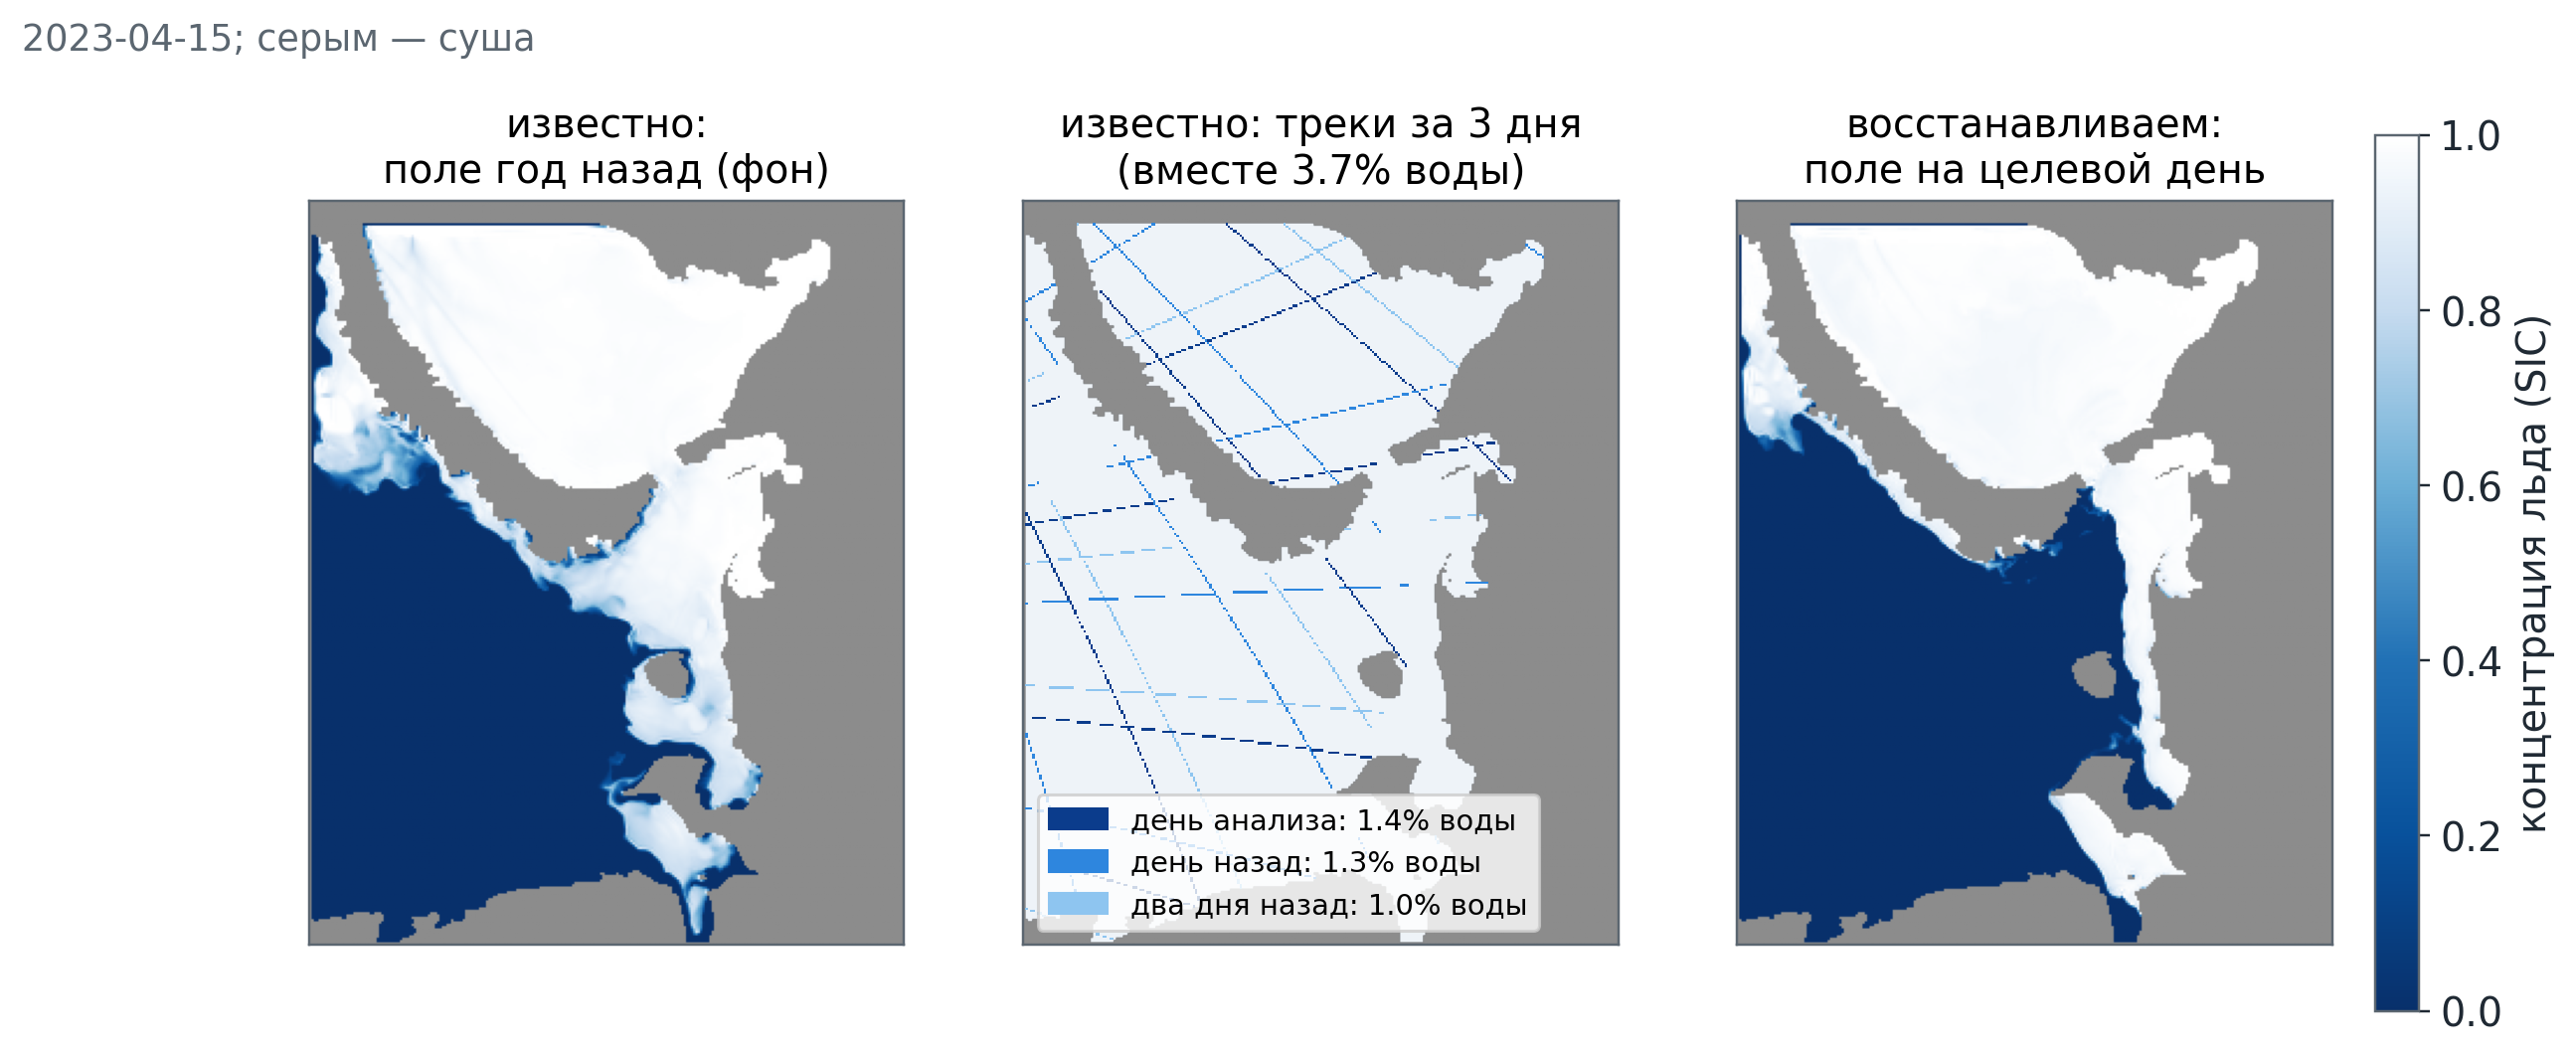
\includegraphics[height=.47\textheight]{figs/ice_setup.png}
\end{frame}

\begin{frame}{Conditional flow matching}
\small
\begin{itemize}
\item Путь от шума к полю: $x_t=(1-t)\,\xi+t\,x$, $\xi\sim\mathcal N(0,I)$, $t\in[0,1]$.
\item Сеть $v_\theta(x_t,t,c)$ обучается на $\E\,\|v_\theta-(x-\xi)\|^2$; оптимум --- $\E[x-\xi\mid x_t,c]$.
\item Условие $c$: фон, значения и маски наблюдений, маска воды, координатная сетка.
\item Генерация: ОДУ $\dot x=v_\theta$ от $t=0$ до $t=1$ (Heun, 32 шага); 16 членов ансамбля из 16 начальных шумов.
\item Сеть --- U-Net; около половины обучающих примеров --- синтетические треки.
\item Данные: обучение 2016--2021, выбор модели 2022, тест 2023.
\end{itemize}
\end{frame}

\begin{frame}{Обычный flow matching плохо использует треки}
\centering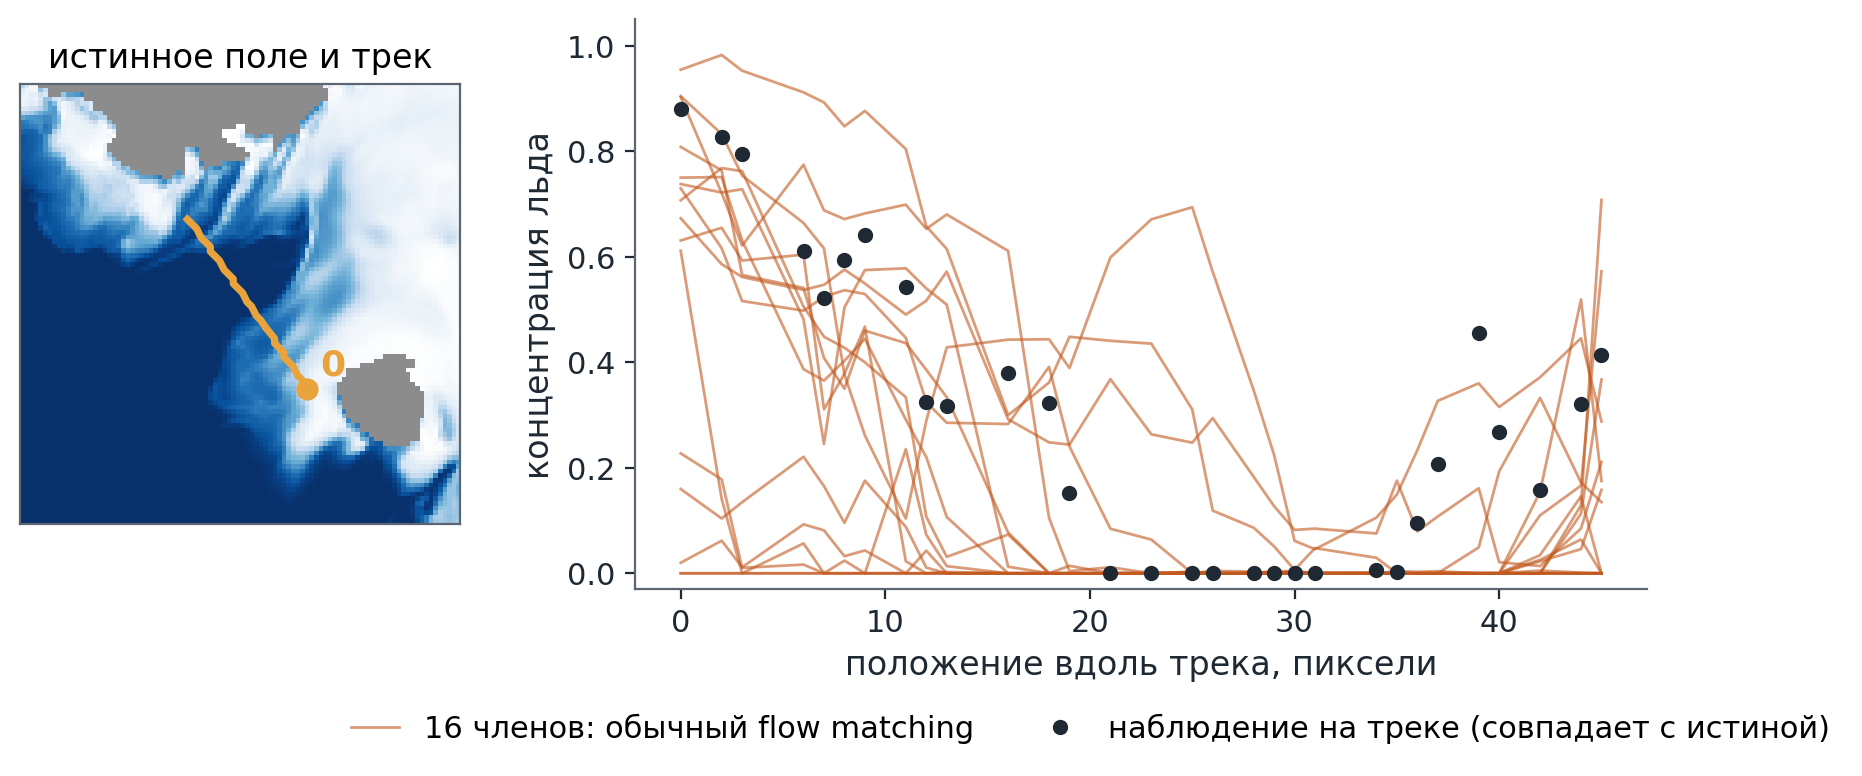
\includegraphics[width=.76\linewidth]{figs/ice_track_problem.png}
\raggedright\small
\begin{itemize}
\item Значение на треке задано точно, но члены ансамбля проходят мимо него: ошибка на треках .12, вдали от треков .23.
\item Треки --- около 4\% пикселей воды, и их вклад в функцию потерь мал.
\item Это не нехватка информации: среднее идеального генератора --- байесовская оценка, и оно не хуже простой копии наблюдения (RMSE .064). У сети --- .124.
\end{itemize}
{\scriptsize\color{ink} 2022 год, точные наблюдения: значение на треке совпадает с истиной. Ошибка --- RMSE одного члена, среднее по 14 дням.\par}
\end{frame}

\begin{frame}{Растянутая шкала концентрации}
\begin{columns}[T]
\begin{column}{.52\textwidth}
\small
Около 55\% пикселей воды --- ровно 0, плотный пак сосредоточен у 1. Непрерывный генератор размазывает ноль в малые положительные значения и выносит пак за 1.

\medskip
Поэтому концентрация генерируется в растянутой шкале
\[z=\tfrac14\,\mathrm{logit}\Big(\frac{\mathrm{SIC}+\varepsilon}{1+2\varepsilon}\Big),\qquad \varepsilon=10^{-3},\]
\[\mathrm{SIC}=\mathrm{clip}\big((1+2\varepsilon)\,\sigma(4z)-\varepsilon,\ 0,\ 1\big).\]
Края шкалы растянуты: значения у 0 и у 1 далеко разнесены. Всё, что сеть выдала ниже образа нуля, переходит ровно в 0.
\end{column}
\begin{column}{.44\textwidth}
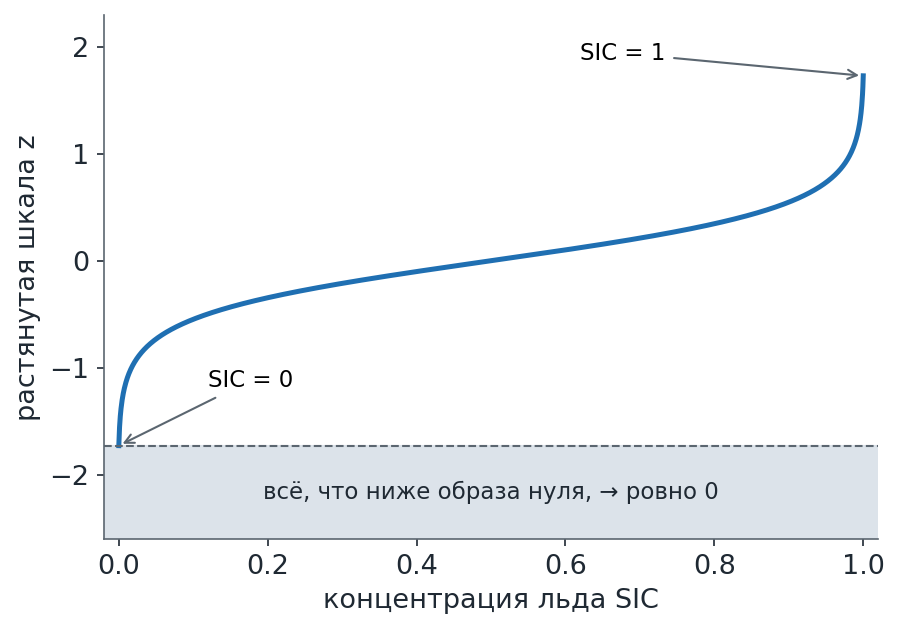
\includegraphics[width=\linewidth]{figs/ice_logit.png}
\end{column}
\end{columns}
\end{frame}

\begin{frame}{Координаты, привязанные к наблюдениям (OA-FM)}
\small
\textbf{Мотивация.} Ширина апостериорного распределения $z$ на треке равна ошибке наблюдения $r\ll1$, вдали от треков --- порядка 1. Поле скоростей должно сжимать ансамбль в $1/r$ раз на 4\% пикселей, и обученная сеть этого не делает.

\textbf{Идея.} Генерировать нормированное отклонение от гауссовой оценки по ближайшему треку:
\[u=\frac{z-m}{s},\qquad m=\rho\,\tilde y,\qquad s=\sqrt{1-\frac{\rho^2}{1+r^2}},\qquad \rho=e^{-d/\ell}.\]
Это оптимальная интерполяция для поля $\mathcal N(0,1)$, коррелированного с треком с коэффициентом $\rho$; $d$ --- расстояние до трека, $\ell=10$ пикселей.
\begin{columns}[T]
\begin{column}{.5\textwidth}
\begin{itemize}
\item В координатах $u$ условная ширина порядка 1 везде: сжимать ансамбль сети не нужно.
\item Ошибка сети $\delta u$ даёт $\delta z=s\,\delta u$; на треке $s\approx r$ --- наблюдение испортить нельзя.
\item Вдали $\rho\to0$ и $u=z$ --- обычная генерация.
\end{itemize}
\end{column}
\begin{column}{.47\textwidth}
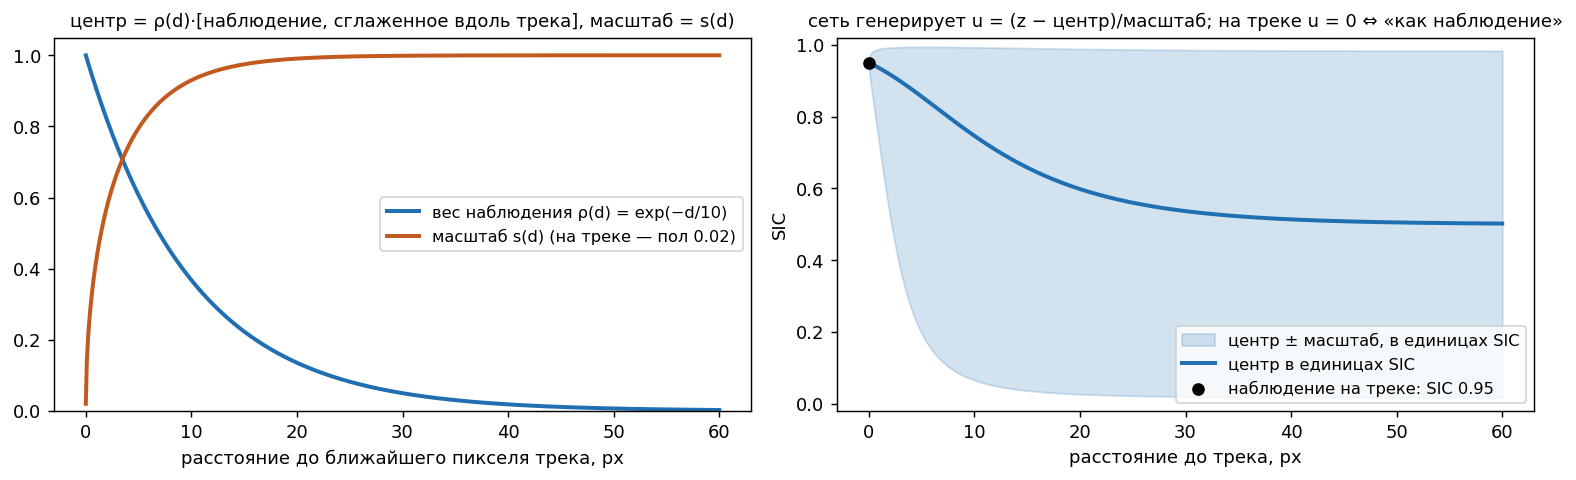
\includegraphics[width=\linewidth]{figs/ice_ap_schematic.png}
\end{column}
\end{columns}
\end{frame}

\begin{frame}{У трека: обычный flow matching и OA-FM}
\centering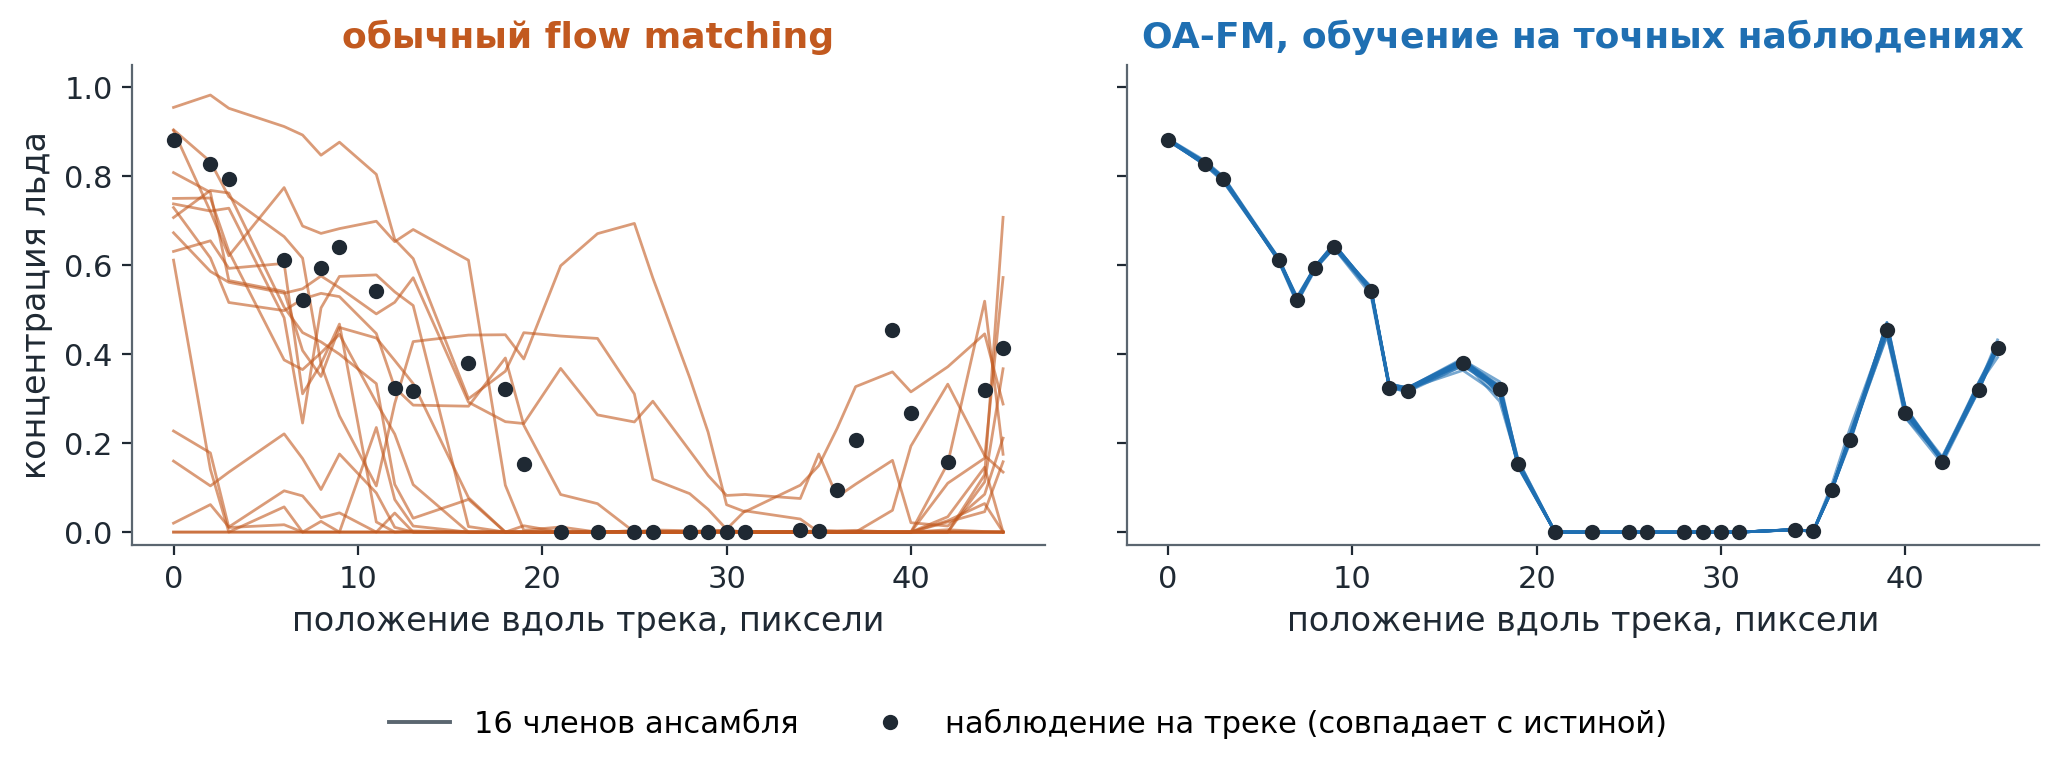
\includegraphics[width=.84\linewidth]{figs/ice_track_fixed.png}
\raggedright\small
\begin{itemize}
\item Тот же трек: все 16 членов OA-FM проходят через наблюдение. Ошибка на треках .12 $\to$ .001, вдали от треков .23 $\to$ .17.
\item Если учить на точных наблюдениях, ансамбль на треках становится слишком уверенным (SSR .03); обучение с моделью ошибки наблюдений даёт SSR .65.
\end{itemize}
\take{Во второй части та же идея --- якорные координаты --- на ERA5. Там видно и то, чего она не решает.}
\end{frame}


% ============================ PART 2 ============================
\begin{frame}[plain]
\vfill
\begin{center}
{\Large\bfseries Часть 2. Как учесть точность наблюдений: метод OSG}\\[4mm]
{\color{ink} ERA5: реальная сеть станций, синтетические наблюдения}
\end{center}
\vfill
\end{frame}

\begin{frame}{Задача: анализ как апостериорное распределение}
\begin{columns}[T]
\begin{column}{.55\textwidth}
\begin{itemize}
\item Есть \textbf{фон} $x_b$ --- прогноз на 24~ч, и \textbf{наблюдения} $y = Hx + \varepsilon$ в отдельных точках ($H$ выбирает наблюдаемые величины).
\item Ошибка наблюдений известна: $\varepsilon\sim\mathcal N(0,R)$. $R$ --- насколько можно верить каждому прибору и как связаны ошибки соседних.
\item Нужен \textbf{ансамбль} из апостериора $p(x\mid x_b,y)$: среднее --- лучшая оценка, разброс --- неопределённость.
\item $R$ меняется: другие приборы, другая точность, коррелированные ошибки. Генеративная модель должна \textbf{правильно} на это реагировать.
\end{itemize}
\end{column}
\begin{column}{.43\textwidth}
\begin{center}
\begin{tikzpicture}[x=1cm,y=1cm]
\node[inp,text width=2.3cm] (b) at (0,.75) {фон $x_b$ (прогноз)};
\node[inp,text width=2.3cm] (y) at (0,-.75) {наблюдения $y$, известная $R$};
\node[box,draw=accent,text width=2.2cm] (a) at (3.6,0) {анализ: ансамбль $x^{(1)},\dots,x^{(M)}$};
\draw[arr] (b.east)--(a.west);
\draw[arr] (y.east)--(a.west);
\end{tikzpicture}
\end{center}
\vspace{2mm}
{\small\color{ink} Главный вопрос: \textbf{как $R$ должна попадать в генеративную модель}.}
\end{column}
\end{columns}
\end{frame}

\begin{frame}{Данные: ERA5, прогноз-фон и сеть станций}
\centering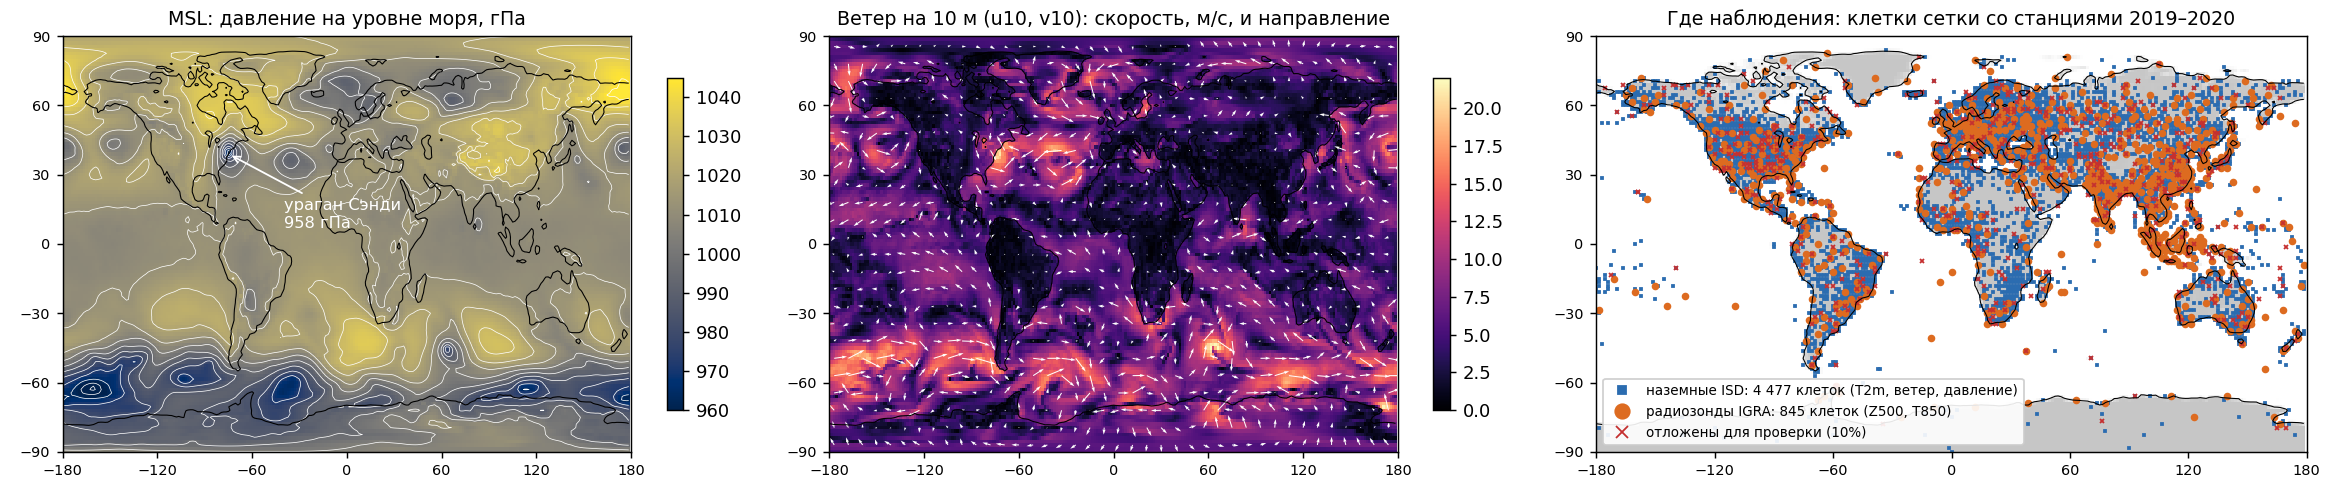
\includegraphics[width=.86\linewidth]{figs/era5_strip.png}\par
{\scriptsize\color{ink} 30 октября 2012: давление у поверхности (ураган Сэнди), ветер у земли и клетки сетки со станциями.\par}
\vspace{1mm}
\raggedright
\begin{columns}[T]
\begin{column}{.5\textwidth}
\footnotesize
\begin{itemize}
\item \textbf{Поле} $x$: ERA5, сетка $1.5^\circ$ ($121\times240$), 6 величин: z500, t850, t2m, ветер u10/v10, давление msl.
\item \textbf{Фон} $x_b$: прогноз на 24~ч нейросетевым эмулятором погоды (UNet) от истинного состояния сутки назад. Ошибка: z500 $\approx$15~м, t850 1.1~K, t2m .9~K, ветер 1.5~м/с, msl 1.5~гПа --- в 3--4 раза меньше, чем у «вчерашнего поля». Оцениваемый год эмулятор не видел.
\end{itemize}
\end{column}
\begin{column}{.48\textwidth}
\footnotesize
\begin{itemize}
\item \textbf{Станции}: фиксированная реальная сеть (радиозонды IGRA, наземные ISD), 19\,598 значений; 10\% клеток отложены для проверки. Наблюдение = правда + шум.
\item \textbf{Шум} сравним с ошибкой фона (z500 $\approx$10~м, t850 1~K, t2m 1.5~K, ветер 1.5~м/с, msl 1~гПа). Точность меняем множителем: «$\sigma\times\lambda$».
\item Обучение 1979--2018, проверка 2019, тест 2020 закрыт.
\end{itemize}
\end{column}
\end{columns}
\end{frame}

\begin{frame}{Два подхода}
\begin{center}
\begin{tikzpicture}[x=1cm,y=1cm,
  b/.style={draw,rounded corners=3pt,align=flush center,inner sep=4pt,font=\small},
  i/.style={b,fill=soft,draw=soft},
  note/.style={anchor=west,align=flush left,text width=3.3cm,font=\footnotesize,text=ink},
  lab/.style={anchor=west,align=flush left,text width=2cm,font=\bfseries}]
\node[lab] at (0,0) {Монолит\\[-1pt]{\footnotesize\mdseries FMPE}};
\node[i,text width=2.1cm] (in1) at (3.25,0) {фон $x_b$,\\наблюдения $y$,\\уровень шума};
\node[b,draw=amr,line width=1pt,text width=4.4cm] (n1) at (7.4,0) {\textbf{одна условная сеть} $p(x\mid y,\sigma,x_b)$, обучена на парах «наблюдения --- поле» с разным шумом};
\node[b,draw=amr,line width=1pt,text width=1.4cm] (o1) at (10.8,0) {ансамбль};
\draw[arr] (in1)--(n1); \draw[arr] (n1)--(o1);
\node[note] at (11.7,0) {шум --- только числом на входе; как его учитывать, сеть учится по примерам};
\node[lab] at (0,-2.1) {OSG\\[-1pt]{\footnotesize\mdseries наш метод}};
\node[i,text width=1.2cm] (in3) at (2.8,-2.1) {фон $x_b$};
\node[b,draw=osg,line width=1pt,text width=1.45cm] (h3) at (4.8,-2.1) {\textbf{голова}\\$h(U\mid x_b)$};
\node[b,draw=osg,line width=1pt,fill=osg!8,text width=1.25cm] (by3) at (6.8,-2.1) {\textbf{точный Байес}};
\node[b,draw=osg,line width=1pt,text width=1.55cm] (k3) at (8.85,-2.1) {\textbf{волокно}\\$K(x\mid U,x_b)$};
\node[b,draw=osg,line width=1pt,text width=1.4cm] (o3) at (10.8,-2.1) {ансамбль};
\node[i,text width=2.1cm] (y3) at (6.8,-3.2) {$y$ и $R$};
\draw[arr] (in3)--(h3); \draw[arr] (h3)--(by3); \draw[arr] (by3)--node[above,font=\footnotesize]{$U$}(k3); \draw[arr] (k3)--(o3); \draw[arr] (y3)--(by3);
\node[note] at (11.7,-2.1) {$R$ --- в точной формуле; генератор $K$ не видит ни $y$, ни $R$};
\end{tikzpicture}
\end{center}
\vspace{-2mm}
{\scriptsize \textbf{На чём учились.} У всех одна архитектура (UNet, 19 млн параметров), те же годы (1979--2018), фоны и сети станций. \textbf{Монолит}: \textbf{одна сеть на все уровни шума}; пары «наблюдения + уровень шума $\to$ поле», шум $=\sigma_0\cdot\lambda$ со случайным $\lambda$ от .03 до 1, $\lambda$ подаётся на вход числом. \textbf{OSG}: $K$ --- на парах «истинные $U$ --- истинное поле», без шума. $U$ --- значения в клетках фиксированной сети станций (19\,598 чисел).\par}
\end{frame}

\begin{frame}{OSG: идея}
Наблюдения зависят от поля \textbf{только через значения в станциях} $U$: $\;y=HU+\varepsilon$. Тогда по формуле Байеса апостериор \textbf{точно} раскладывается на два множителя:
\[
p(x\mid x_b,y)\;=\;\underbrace{p(U\mid x_b,y)}_{\substack{\text{станции:}\\ \text{вся информация о } y \text{ и } R}}\;\cdot\;\underbrace{p(x\mid U,x_b)}_{\substack{\text{поле по станциям:}\\ \text{о } y \text{ и } R \text{ не знает}}}
\]
\begin{columns}[T]
\begin{column}{.55\textwidth}
\begin{itemize}
\item \textbf{Первый множитель} --- маленькая задача в станциях: гауссов prior + известная $R$ = точная формула для \textbf{любой} $R$.
\item \textbf{Второй множитель} --- генеративная модель $K$: как достроить поле по точным значениям в станциях. Учится один раз на парах «истинные $U$ --- истинное поле», без шума наблюдений.
\end{itemize}
\end{column}
\begin{column}{.42\textwidth}
\small
\textbf{Почему это верно.} $p(x\mid x_b,y)\propto p(y\mid U)\,p(x\mid x_b)$ и $p(x\mid x_b)=p(U\mid x_b)\,p(x\mid U,x_b)$. Множитель $p(y\mid U)$ касается только $U$:
\[p(x\mid x_b,y)\propto \big[p(y\mid U)\,p(U\mid x_b)\big]\,p(x\mid U,x_b).\]
{\color{ink}Это не приближение: если голова и $K$ точны, ансамбль OSG --- точный апостериор при любой $R$.}
\end{column}
\end{columns}
\end{frame}

\begin{frame}{OSG: три шага}
\centering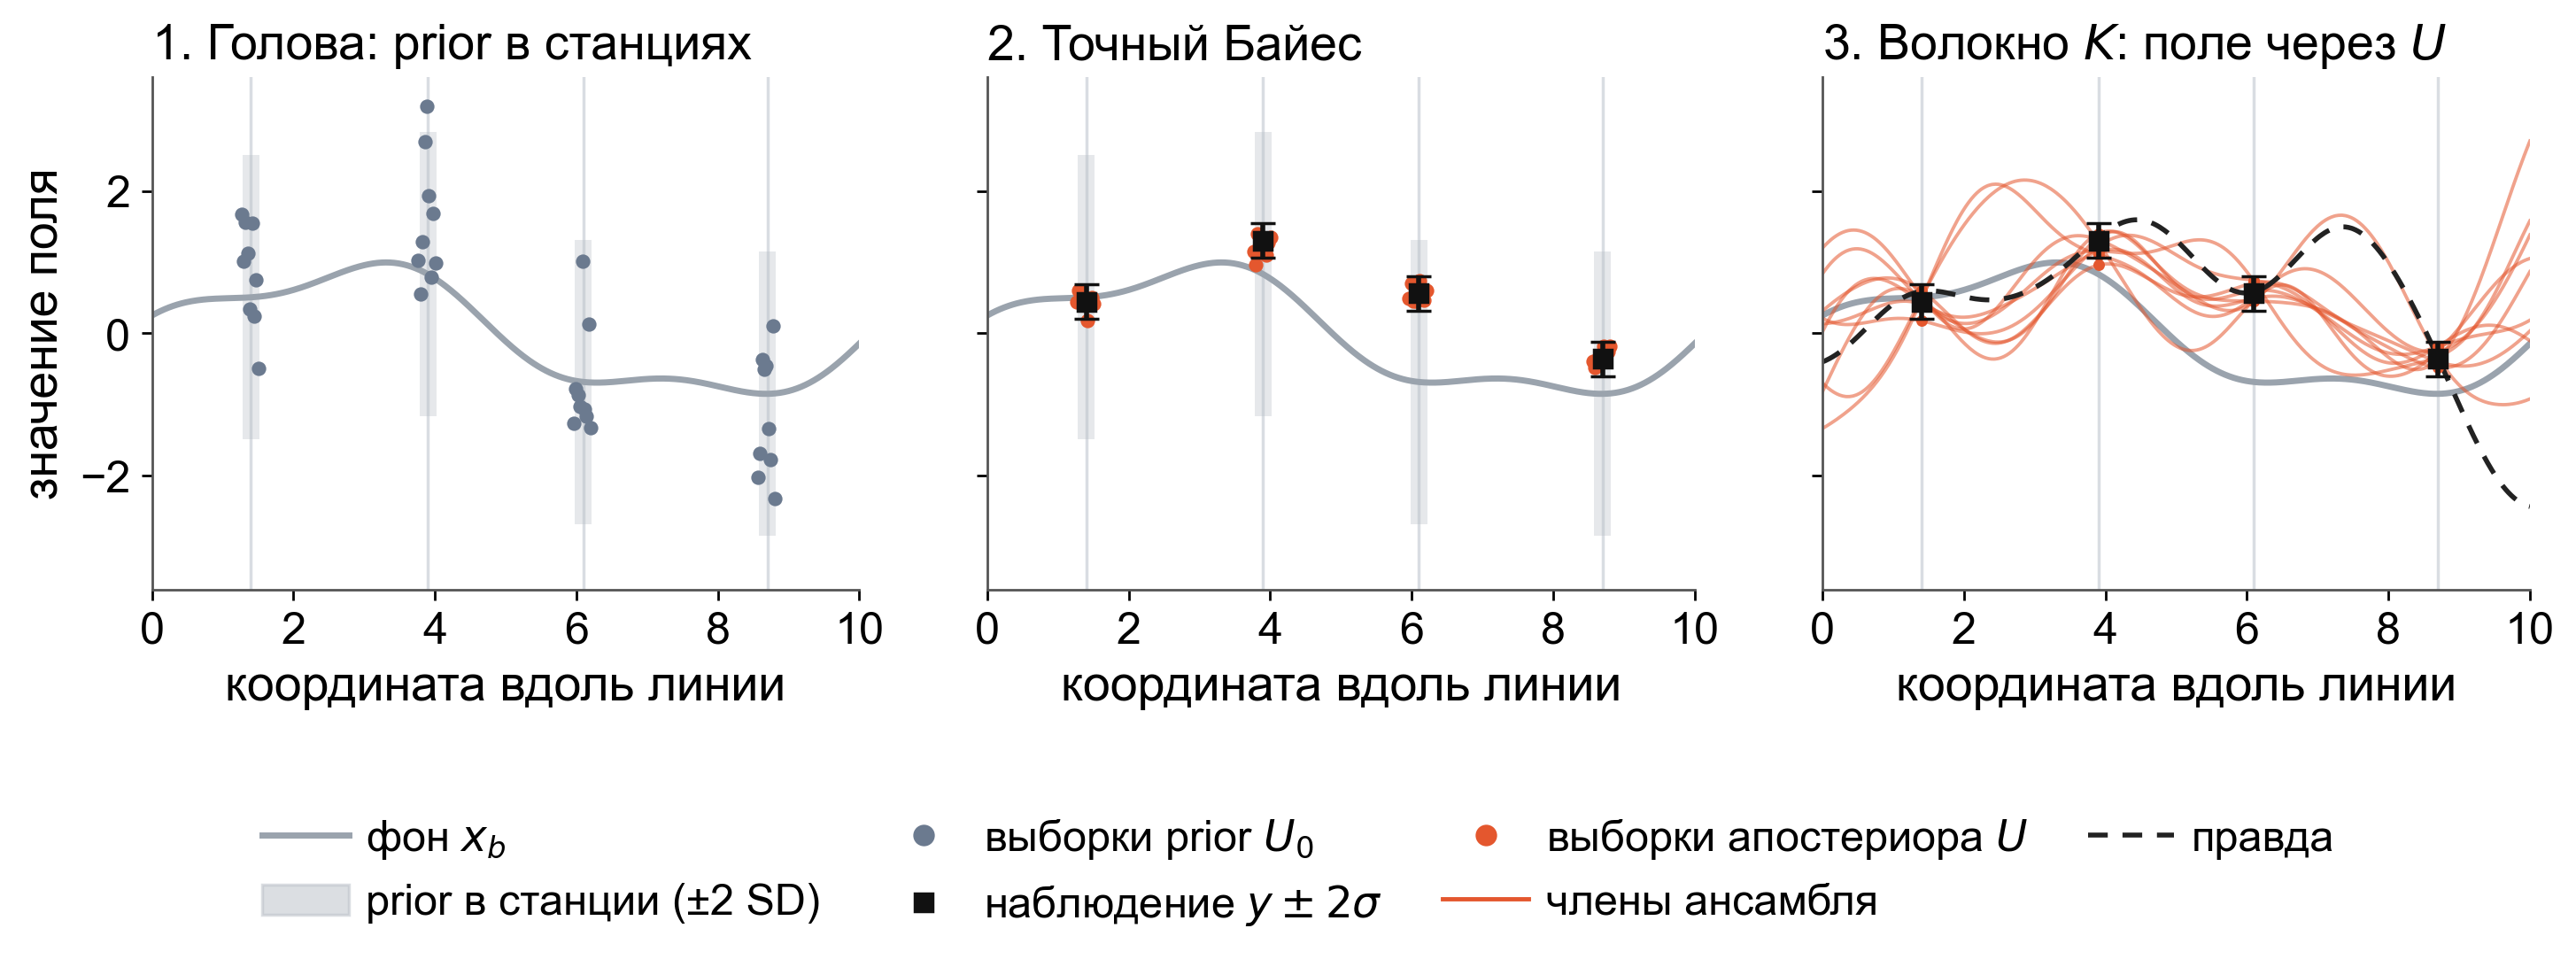
\includegraphics[width=.84\linewidth]{figs/osg_idea.png}\par
{\scriptsize\color{ink} Иллюстрация на гауссовом процессе, а не на ERA5.\par}
\raggedright\footnotesize
\begin{enumerate}
\item \textbf{Голова} $h(U\mid x_b)$: гауссов prior в станциях по всему полю фона (подробнее --- следующий слайд).
\item \textbf{Точный Байес} (правило Матерона): $U=U_0+CH^\top(HCH^\top+R)^{-1}(y+\varepsilon-HU_0)$, $U_0\sim h$, $\varepsilon\sim\mathcal N(0,R)$ --- точная выборка апостериора; тот же шаг, что в EnKF, но только в станциях.
\item \textbf{Волокно} $K(x\mid U,x_b)$: генерирует остальное поле как приращение к фону. Значения в станциях оно \textbf{не генерирует, а закрепляет} --- сжимать ансамбль сети не нужно. Это выборки шага 2: у каждого члена свои $U$, шум наблюдений уже учтён.
\end{enumerate}
\end{frame}

\begin{frame}{Голова $h(U\mid x_b)$: чего ждать от ошибки фона в станциях сегодня}
\begin{columns}[T]
\begin{column}{.55\textwidth}
\small
Гауссово распределение для 19\,598 значений в станциях, в единицах приращения $a=(U-x_b)/s_b$: \textbf{насколько и как фон ошибается в станциях в этот срок}. Аналог матрицы $B$ из 3D-Var, но только в станциях и зависящий от погоды:
\[
a\sim\mathcal N\big(\mu+\delta,\;\; D\,C_L\,D+F F^\top\big).
\]
\footnotesize
\begin{itemize}
\item $\mu$, $C_L$ --- статическая часть: средняя ошибка фона и её ковариация по обучающим годам; $C_L$ сглажена локализацией.
\item $\delta$ --- сдвиг: систематическая ошибка фона сегодня.
\item $D$ --- масштабы от .61 до 1.65: где фон сегодня надёжнее или хуже обычного.
\item $F$ --- 16 «погодных мод»: сегодняшние связанные ошибки соседних станций.
\end{itemize}
\end{column}
\begin{column}{.42\textwidth}
\small
\textbf{Откуда $\delta$, $D$, $F$}: их даёт UNet по всему полю фона (плюс рельеф, суша/море, время). Наблюдения $y$ и $R$ на вход \textbf{не подаются}.

\textbf{Обучение}: максимум правдоподобия истинных приращений в станциях (1979--2018).

\textbf{Почему гауссова}: тогда шаг Байеса точный и дешёвый.

\textbf{Что даёт погода}: апостериор в станциях на 12\% точнее по CRPS, чем со статической головой.

{\color{ink}\textbf{Ограничение}: хвосты гауссовы --- на редких больших невязках ($\ge3\sigma$) станции хуже на 2.5--4.6\%.}
\end{column}
\end{columns}
\end{frame}

\begin{frame}{Преимущества OSG}
\begin{columns}[T]
\begin{column}{.6\textwidth}
\begin{itemize}
\item \textbf{Любая $R$ без переобучения}: другая точность, неоднородный шум, коррелированные ошибки --- меняется только формула шага 2.
\item \textbf{Точные наблюдения используются полностью}: при $R\to0$ шаг 2 возвращает наблюдения; сжимать ансамбль генератору не нужно.
\item \textbf{Генератор учится один раз и без шума}.
\item \textbf{Цена как у монолита}: 6.2~с на срок против 5.65~с (16 членов, V100).
\end{itemize}
\end{column}
\begin{column}{.37\textwidth}
\small
\textbf{Ограничения}
\begin{itemize}
\item Голова гауссова: на редких больших невязках станции хуже.
\item Наблюдения --- на фиксированной сети станций ($y=HU+\varepsilon$).
\end{itemize}
\end{column}
\end{columns}
\end{frame}

\begin{frame}{Пример анализа: точные наблюдения ($\sigma\times.1$)}
\centering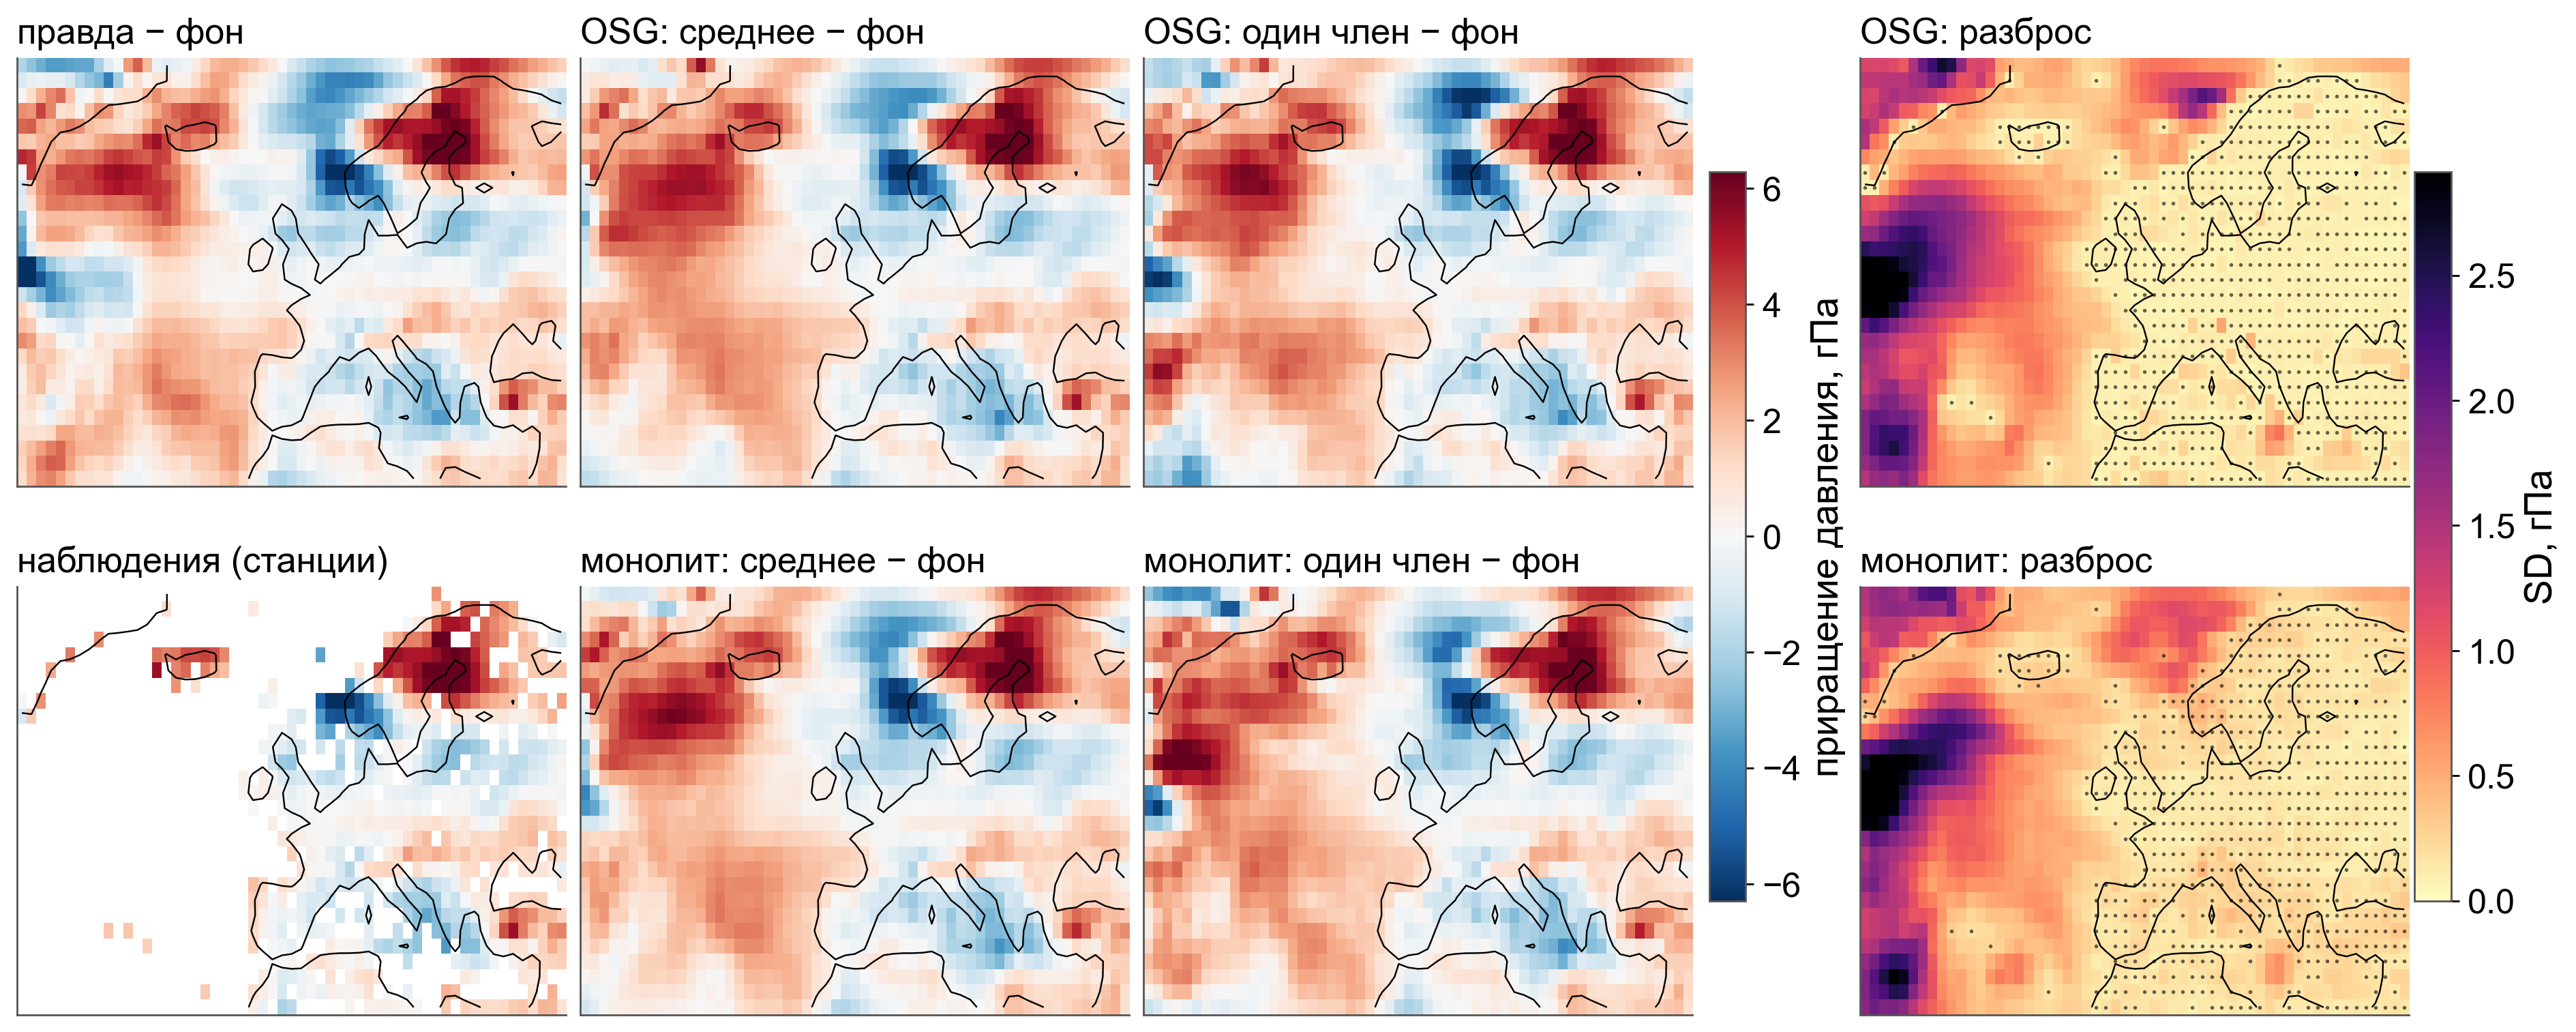
\includegraphics[width=\linewidth]{figs/maps3.png}\par
\raggedright\small
1 января 2019, давление у поверхности, Северная Атлантика и Европа; точки --- станции. Оба метода восстанавливают приращение там, где есть станции; разброс мал над сушей со станциями и велик над океаном. По одной карте методы почти не различить --- разница видна в статистике по 67 срокам.
\end{frame}

\begin{frame}{Результат 1. Точность при разной ошибке наблюдений}
\begin{center}
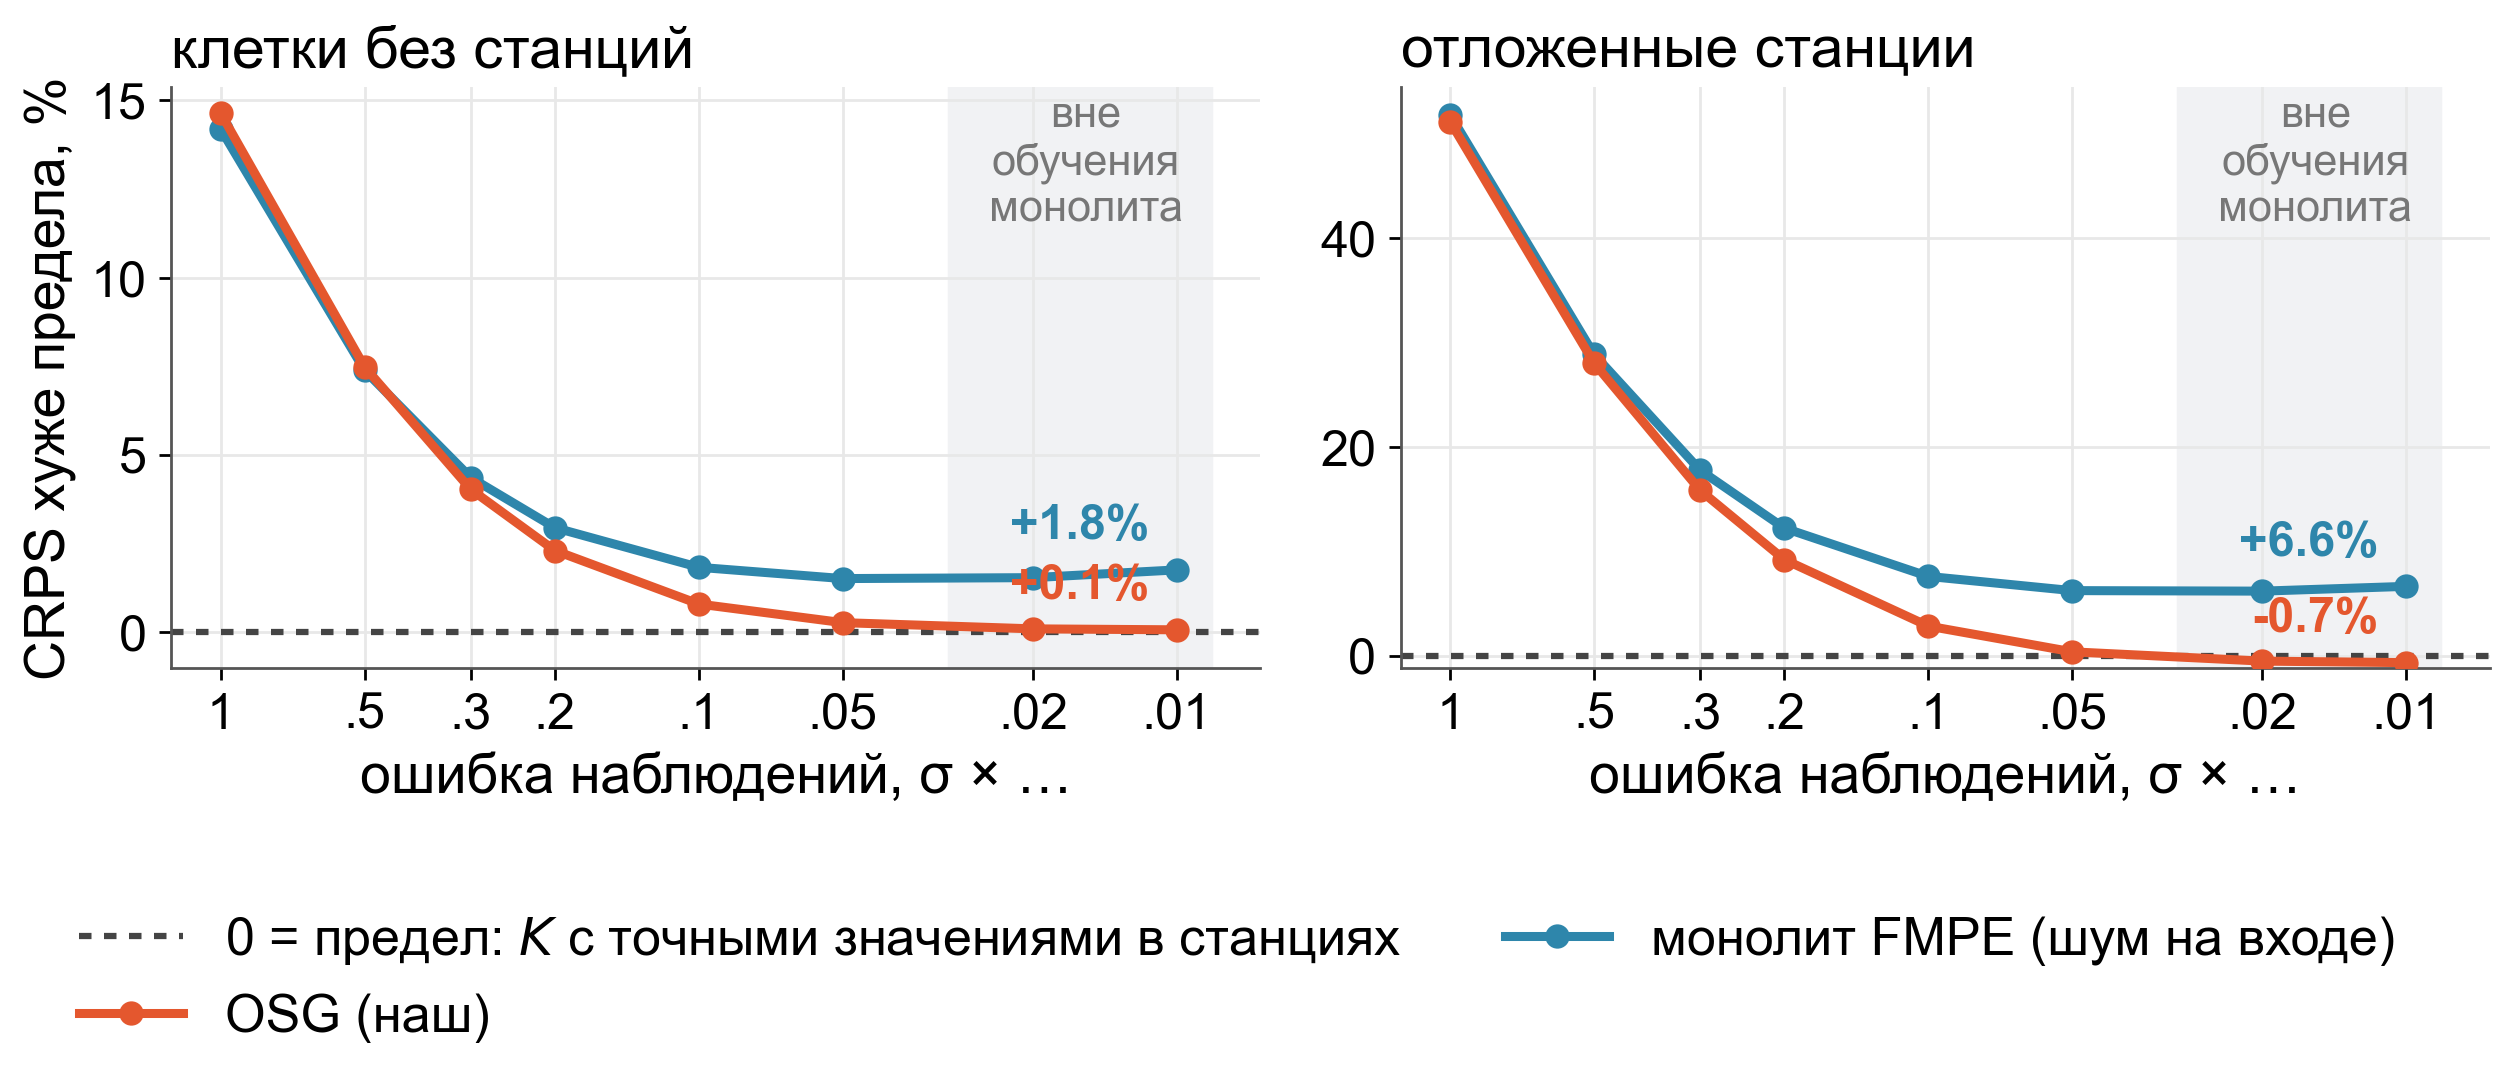
\includegraphics[height=.5\textheight]{figs/precision3.png}
\end{center}
\vspace{-3mm}
\footnotesize
\begin{itemize}
\item \textbf{Как читать}: насколько CRPS хуже \textbf{предела} --- $K$ с точными значениями в станциях (0 --- лучше не бывает).
\item \textbf{Обычная ошибка} ($\sigma\times1$): все на $\approx$15\% хуже предела; монолит точнее OSG на .4\%, но при разной точности станций по регионам OSG лучше на .9\% (монолит видит только общий уровень шума).
\item \textbf{Точные наблюдения}: OSG доходит до предела, монолит застревает выше --- +1.8\% по полю и +6.6\% на отложенных станциях при $\sigma\times.01$.
\end{itemize}
\end{frame}

\begin{frame}{Почему монолит не использует точные наблюдения}
\begin{center}
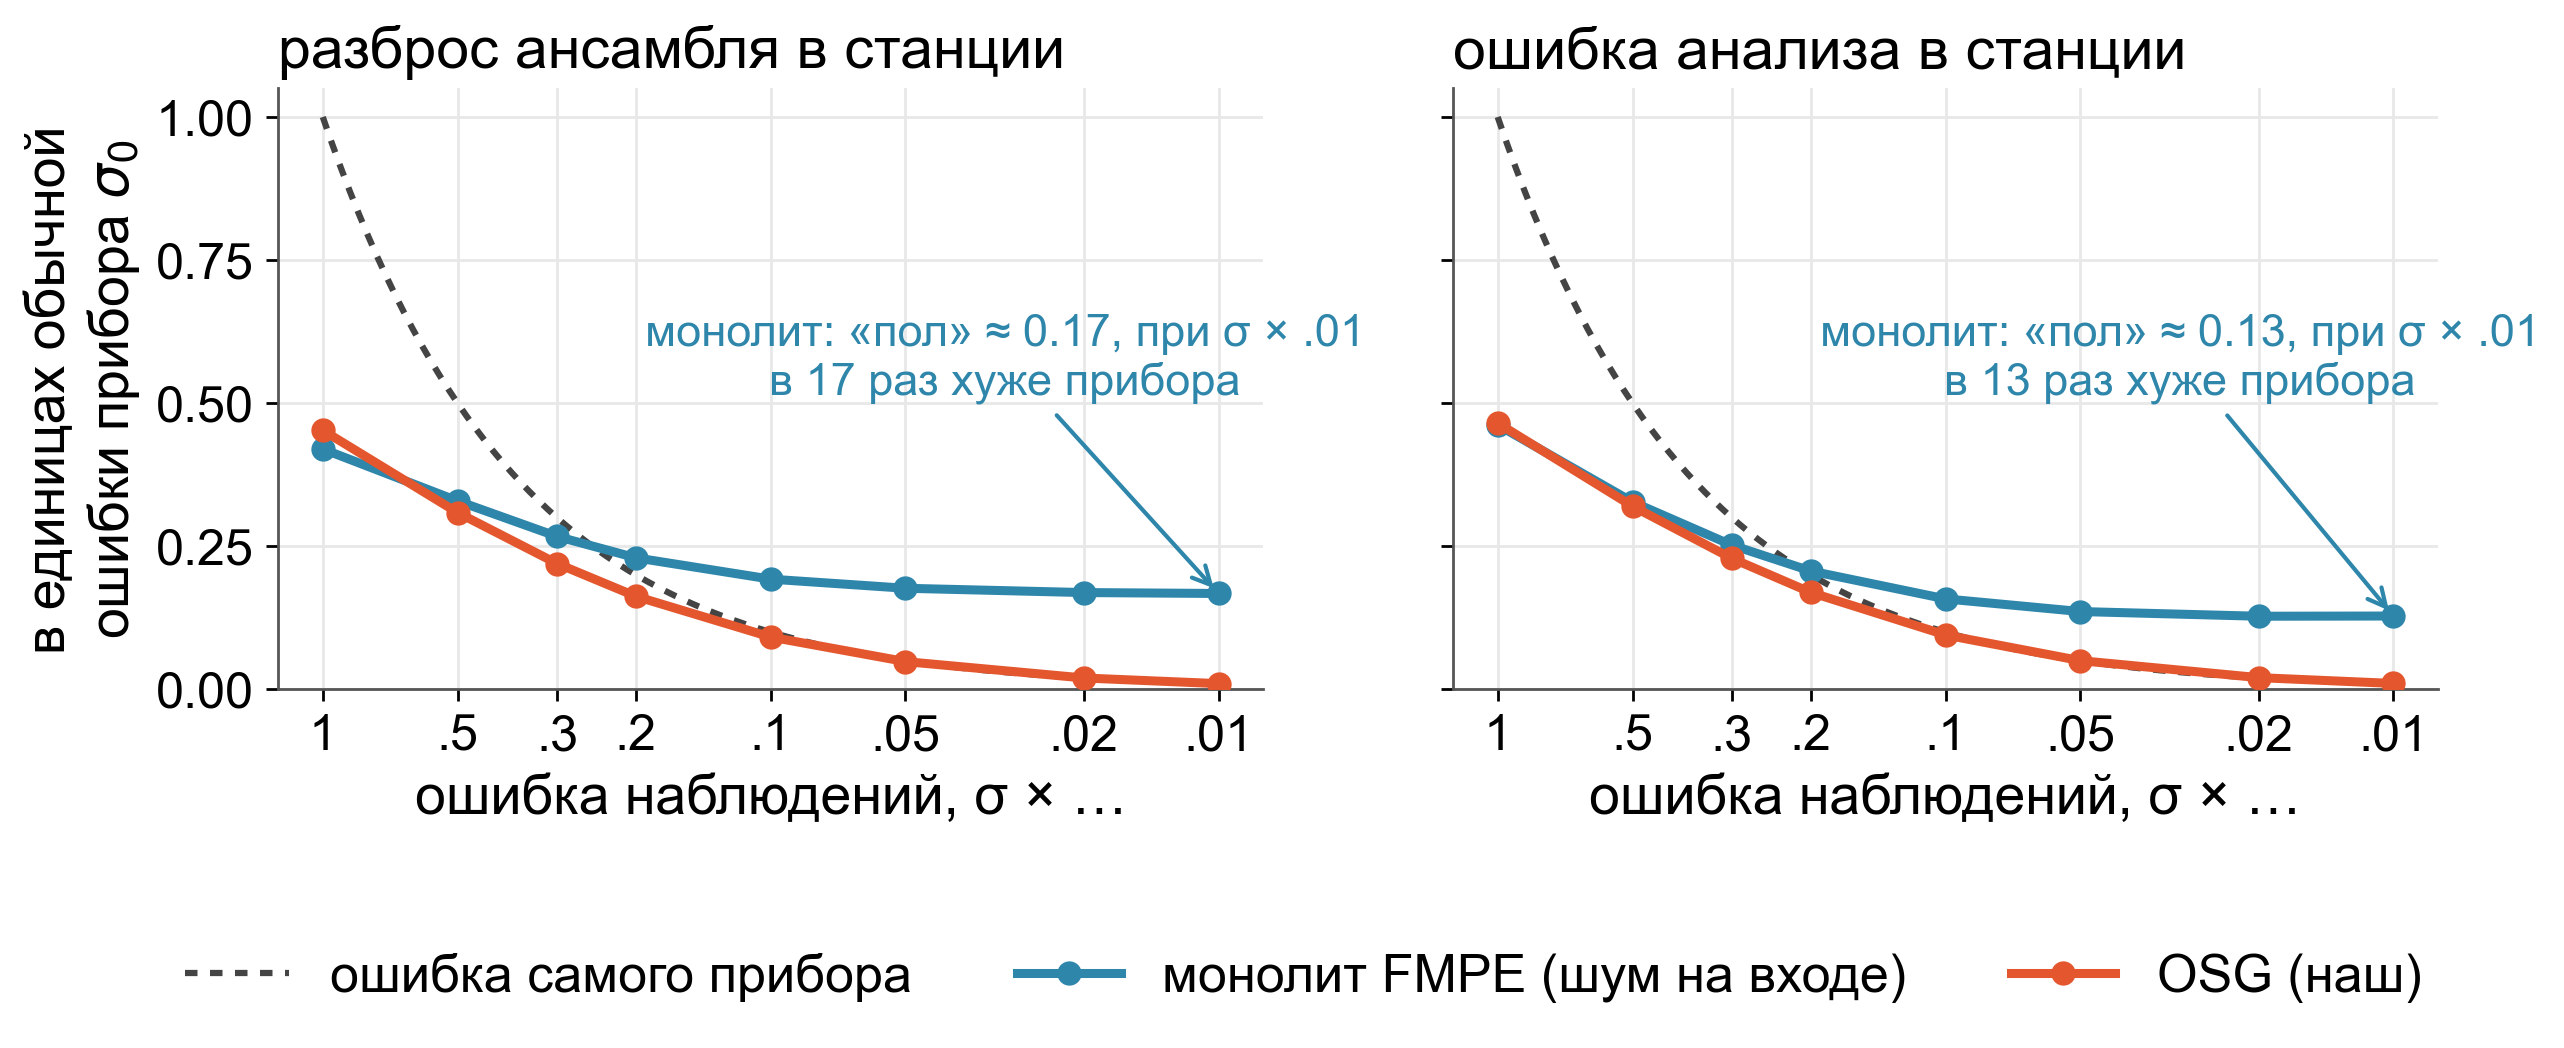
\includegraphics[height=.52\textheight]{figs/stations3.png}
\end{center}
\vspace{-3mm}
\small
\begin{itemize}
\item \textbf{Как читать}: разброс ансамбля и ошибка анализа в самих станциях; пунктир --- ошибка самого прибора. Хороший анализ не хуже прибора: при обычной ошибке лучше (помогают фон и соседние станции), при точных наблюдениях --- на уровне прибора.
\item OSG идёт вниз вместе с прибором (шаг 2). Монолит упирается в «пол» и при $\sigma\times.01$ в 13--17 раз хуже прибора --- та же проблема, что с треками во льду.
\end{itemize}
\end{frame}

\begin{frame}{Результат 2. Калибровка: ранговые гистограммы}
\begin{center}
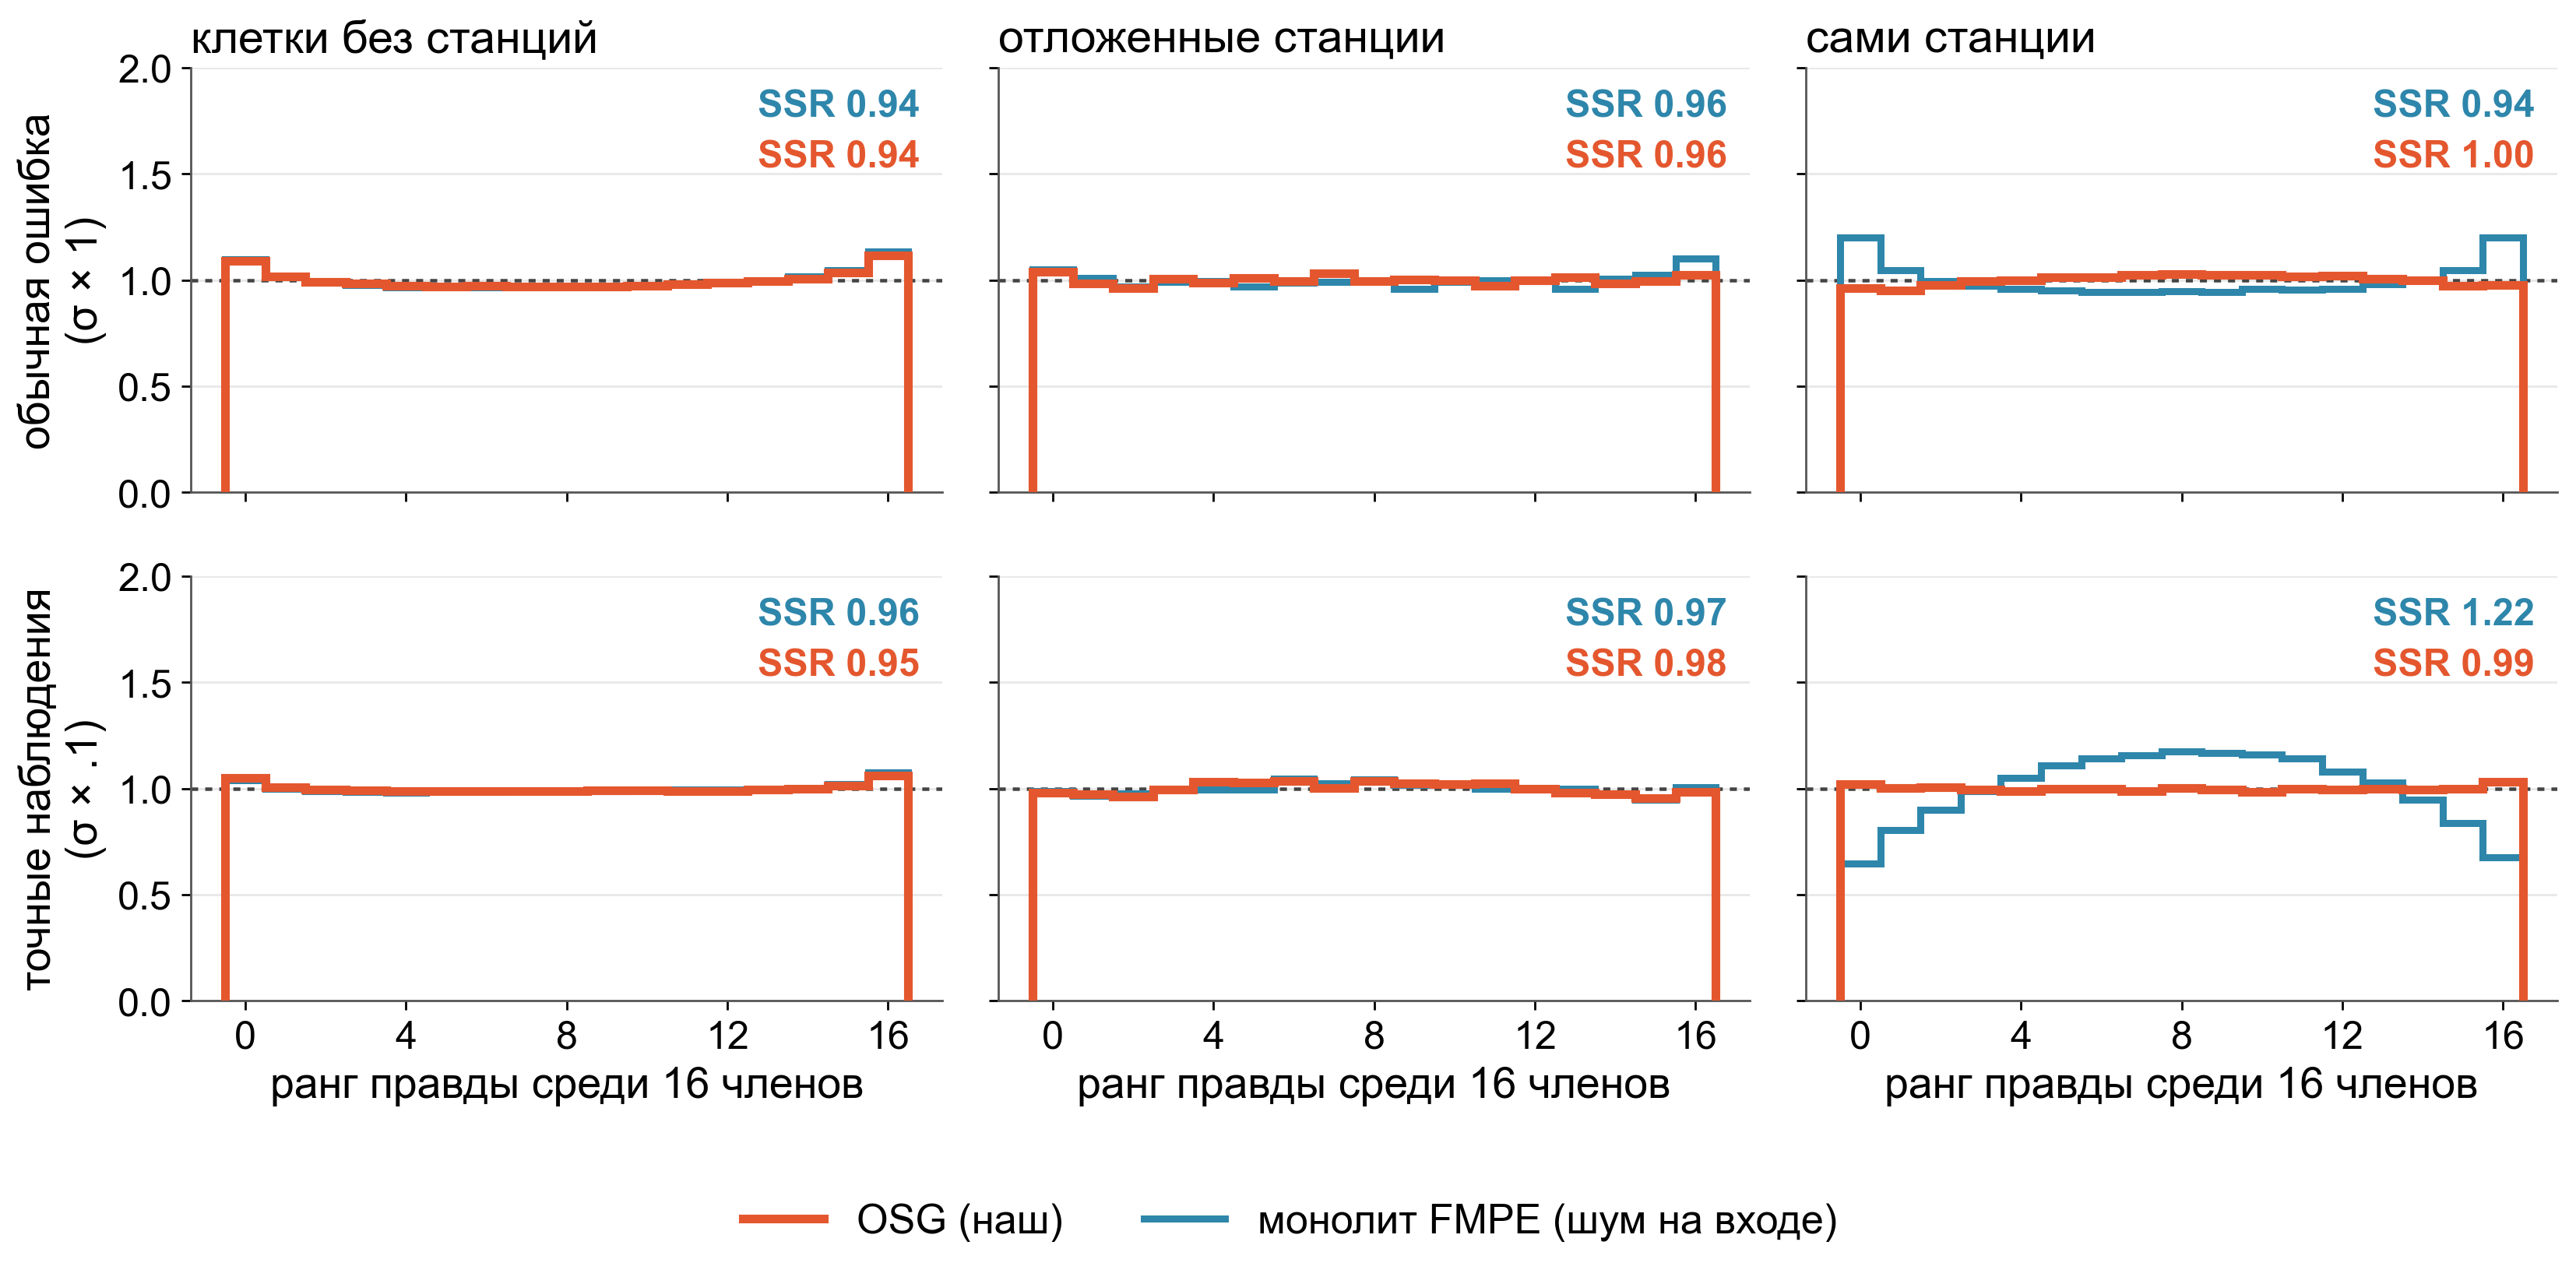
\includegraphics[height=.6\textheight]{figs/ranks3.png}
\end{center}
\vspace{-3mm}
\footnotesize
\begin{itemize}
\item \textbf{Как читать}: ранг правды среди 16 членов. Ровно на уровне 1 --- разброс честный; $\cup$ --- ансамбль слишком уверен; $\cap$ --- слишком широк. SSR --- разброс / ошибка, 1 --- честно.
\item В поле и на отложенных станциях оба метода откалиброваны. В самих станциях монолит --- нет: при обычной ошибке $\cup$, при точных наблюдениях $\cap$ (SSR 1.22) --- он не может сжаться. OSG ровный везде.
\end{itemize}
\end{frame}

\begin{frame}{Результат 3. Коррелированные ошибки наблюдений}
\centering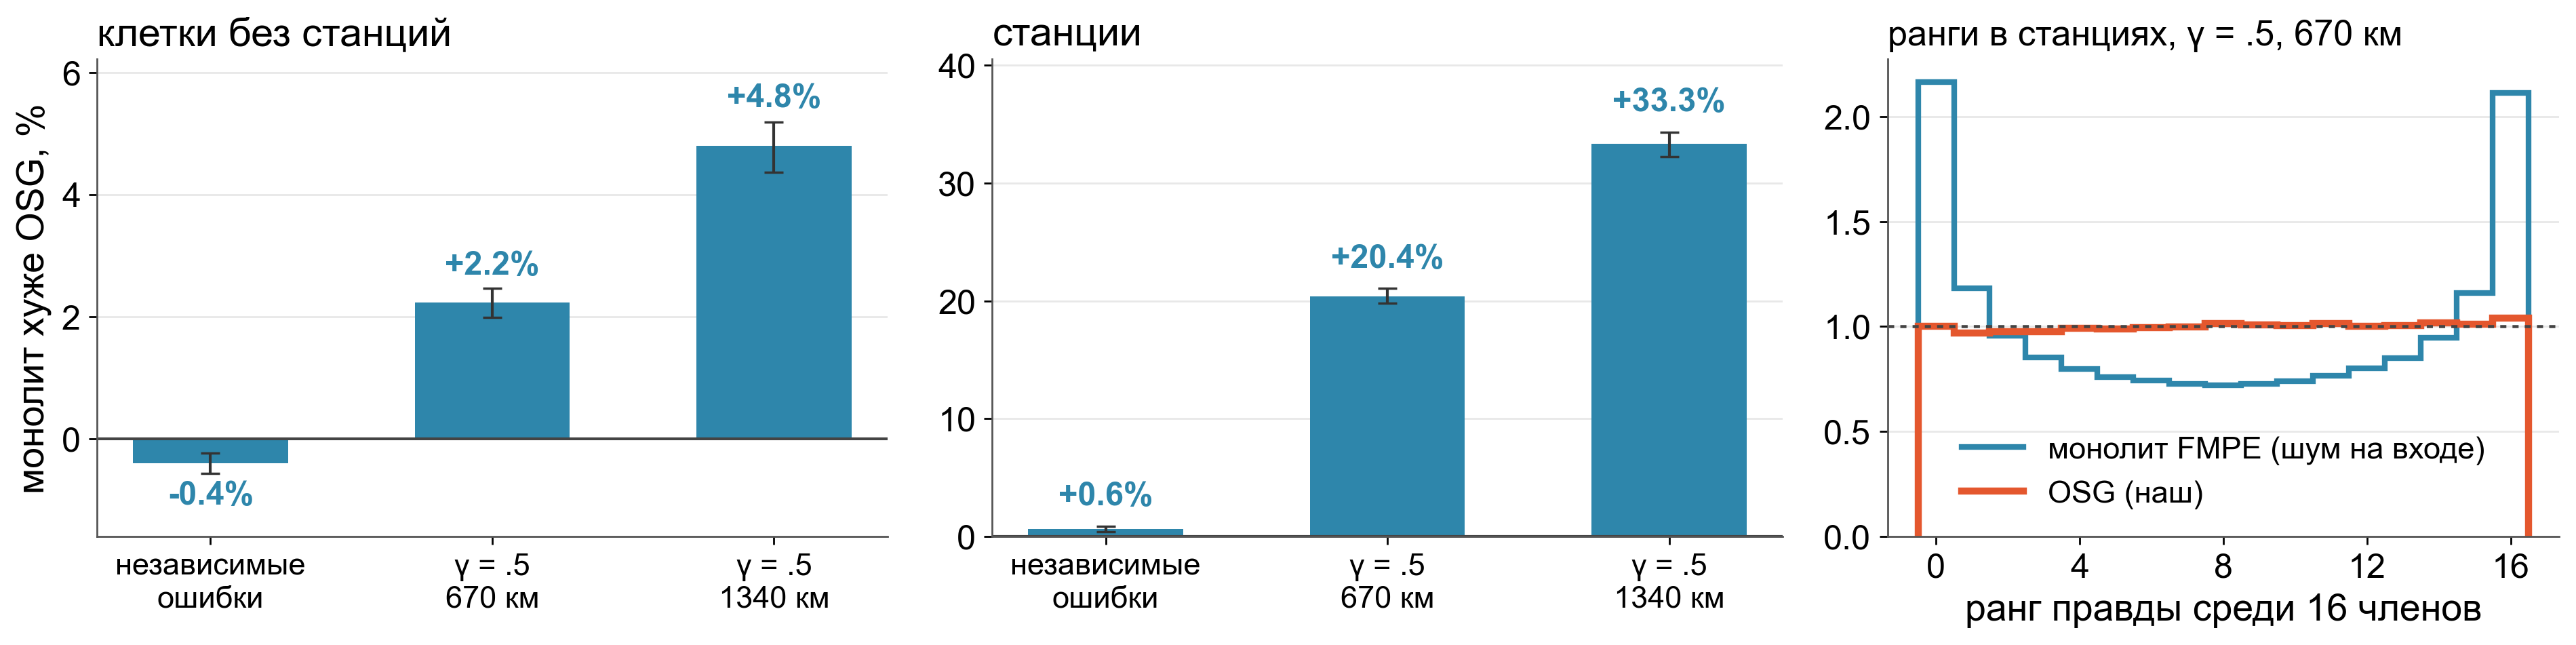
\includegraphics[width=\linewidth]{figs/corr3.png}\par
\raggedright\small
\begin{itemize}
\item Ошибки соседних станций связаны: $R=D[(1-\gamma)I+\gamma C_\ell]D$, $\gamma$ --- доля общей ошибки, длина связи $\approx$670 или 1340~км (модель ошибок задана нами). OSG подставляет полную $R$ в шаг 2, монолит знает только уровень шума.
\item При $\gamma=.5$ монолит хуже OSG на 2.2--4.8\% по полю и на 20--33\% на станциях; в станциях он слишком уверен ($\cup$), OSG ровный.
\item Если монолит \textbf{переобучить} на коррелированных ошибках, по полю он догоняет OSG (паритет на 670~км, OSG лучше на .4\% на 1340~км); OSG точнее в станциях на 1--3\% --- и обходится без переобучения.
\end{itemize}
\end{frame}

\begin{frame}{Итог}
\small
\textbf{Что показали} (ERA5, проверочный 2019 год; OSG против стандартного монолита)
\begin{enumerate}
\item OSG применяет известную ошибку наблюдений точно и без переобучения: генератор учится один раз, $R$ входит формулой.
\item Точные наблюдения: OSG выходит на предел «$K$ с точными значениями в станциях»; стандартный монолит застревает выше (+1.8\% по полю, +6.6\% на отложенных станциях), потому что не умеет сжать ансамбль в станциях: там он в 13--17 раз хуже прибора.
\item Калибровка: OSG ровный везде; монолит в станциях --- нет.
\item Коррелированные ошибки: OSG лучше монолита на 2.2--4.8\% по полю без переобучения; переобученный монолит догоняет его по полю, но не в станциях.
\item Специалист, обученный только на точных наблюдениях, на своём шуме почти догоняет OSG (на .3\%), но на другие уровни шума не переносится.
\end{enumerate}
\textbf{Честно}: при однородном номинальном шуме монолит на .4\% точнее; голова гауссова; сеть станций фиксирована; наблюдения синтетические; тест 2020 ещё не открыт.

\textbf{Дальше}: заморозка и закрытый тест 2020; реальные наблюдения; лёд как второй домен; статья.
\end{frame}

\end{document}
